\section{Maths for 2D motion}
\subsection{Definitions}
\begin{figure}[h!]
	\centering
	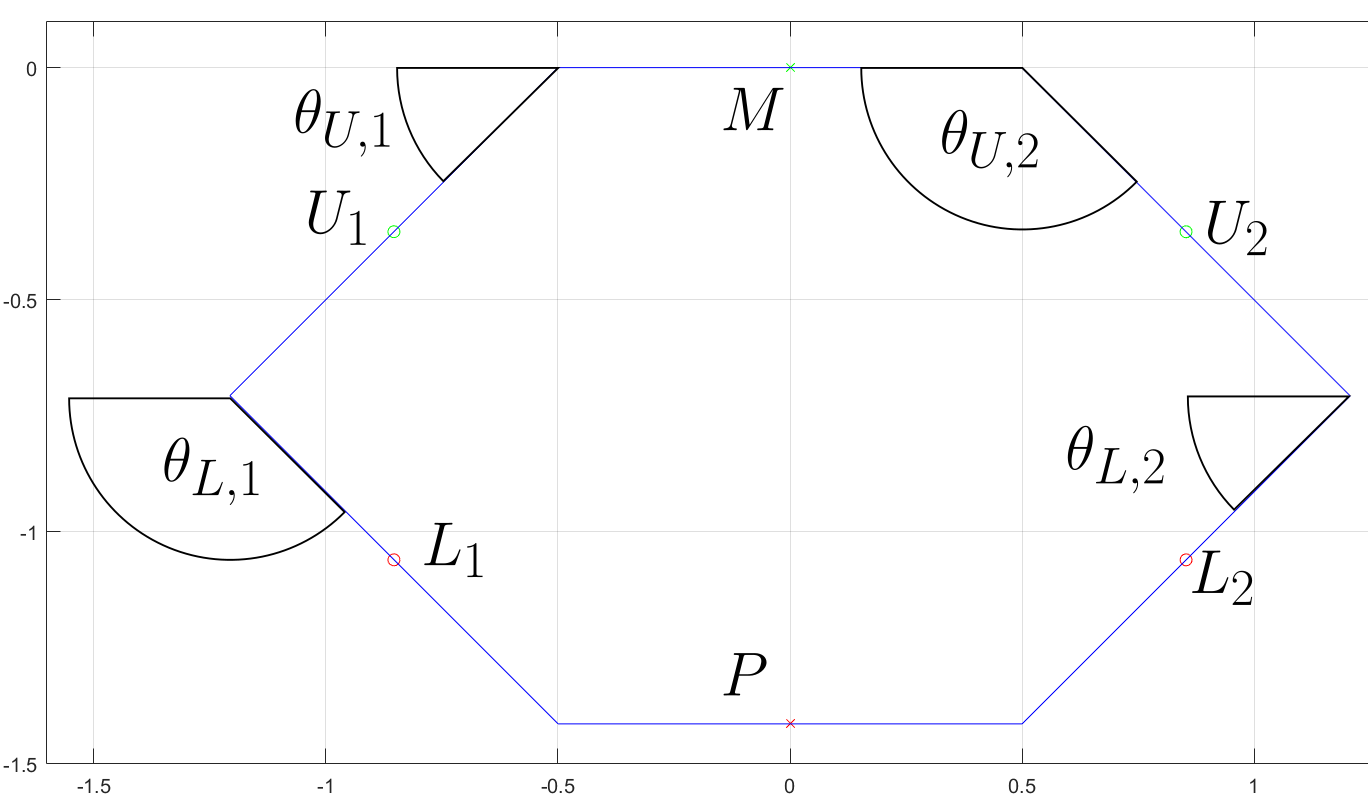
\includegraphics[width=0.7\textwidth]{figures/Initial_2D.png}                                                              
	\caption[Initial configuration of the 2D Delta robot]{Initial configuration of the 2D Delta robot.}
	\label{fig:initial2D}
\end{figure}

Constraint equations
\begin{equation}
    \Phi=
    \begin{bmatrix}
    \begin{array}{l} % for proper alignment
    M_x\mp\frac{L_b}{2}-U_{j,x}-\frac{L_u}{2} cos(\theta_{U,j}) \\
    M_y-U_{j,y}-\frac{L_u}{2} sin(\theta_{U,j})\\
    U_{j,x}-\frac{L_u}{2}cos(\theta_{U,j})-L_{j,x}-\frac{L_l}{2}cos(\theta_{L,j}) \\
    U_{j,y}-\frac{L_u}{2}sin(\theta_{U,j})-L_{j,x}-\frac{L_l}{2}sin(\theta_{L,j})\\
    L_{j,x}-\frac{L_l}{2}cos(\theta_{L,j})-P_x \pm \frac{L_e}{2} \\
    L_{j,y}-\frac{L_l}{2}sin(\theta_{L,j})-P_y%\\
    %\theta_{U,j} - \omega_i t - (\theta_{U,j})_0
    \end{array}\\
    \vdots \\
    \vdots
    \end{bmatrix}
    \label{eq:Phi2D}
\end{equation}

\begin{equation}
    \Phi^{driving}=
    \begin{bmatrix}
    \theta_{U,1} - \omega_1 t - (\theta_{U,1})_0\\
    \theta_{U,2} - \omega_2 t - (\theta_{U,2})_0
    \end{bmatrix}
\end{equation}

Independent and Dependent Co-ordinates
\begin{align}
    q_i&=
    \begin{bmatrix}
    \theta_{U,1} \\
    \theta_{U,2}
    \end{bmatrix} &
    q_d&=
    \begin{bmatrix}
    \; \; \vdots \; \;
    \end{bmatrix}
\end{align}

\subsection{Kinematics}
\begin{align}
            \Phi &= 0  \nonumber \\
\implies \tfrac{d\Phi}{dt} &=\Phi_q \tfrac{dq}{dt}+ \Phi_t =0 \label{eq:PhiDot} \\
\therefore \tfrac{dq}{dt}&=-\Phi_q^{-1} \Phi_t \\
\implies \tfrac{d^2\Phi}{dt^2} &=([\Phi_{q}\tfrac{dq}{dt}]_q\tfrac{dq}{dt}+[\Phi_{q}\tfrac{dq}{dt}]_t)+(\Phi_{tq}\tfrac{dq}{dt}+\Phi_{tt})=0 \label{eq:PhiDDot} \\
\therefore  \tfrac{d^2q}{dt^2}&=-\Phi_q^{-1} (\Phi_{qq}\tfrac{dq}{dt}^2+2\Phi_{qt}\tfrac{dq}{dt}+\Phi_{tt}) \nonumber \\
                    &=\Phi_q^{-1} \gamma \label{eq:Gamma}
\end{align}

%%Embedded form:
%\begin{align}
%         J&=\Phi_{q_d}^{-1}\Phi_{q_i} \\
% \dot{q}_d&=-J\dot{q}_i\\
%   \hat{M}&=M_{ii}+ J^T M_{dd}J\\
%   \hat{Q}&=-J^T Q_{A,d}+J^T M_{dd}\Phi_{q_d}^{-1}\gamma
%\end{align}

\subsection{Inverse Kinematics}
\label{sec:Inverse2D}

\begin{figure}[h!]
	\centering
	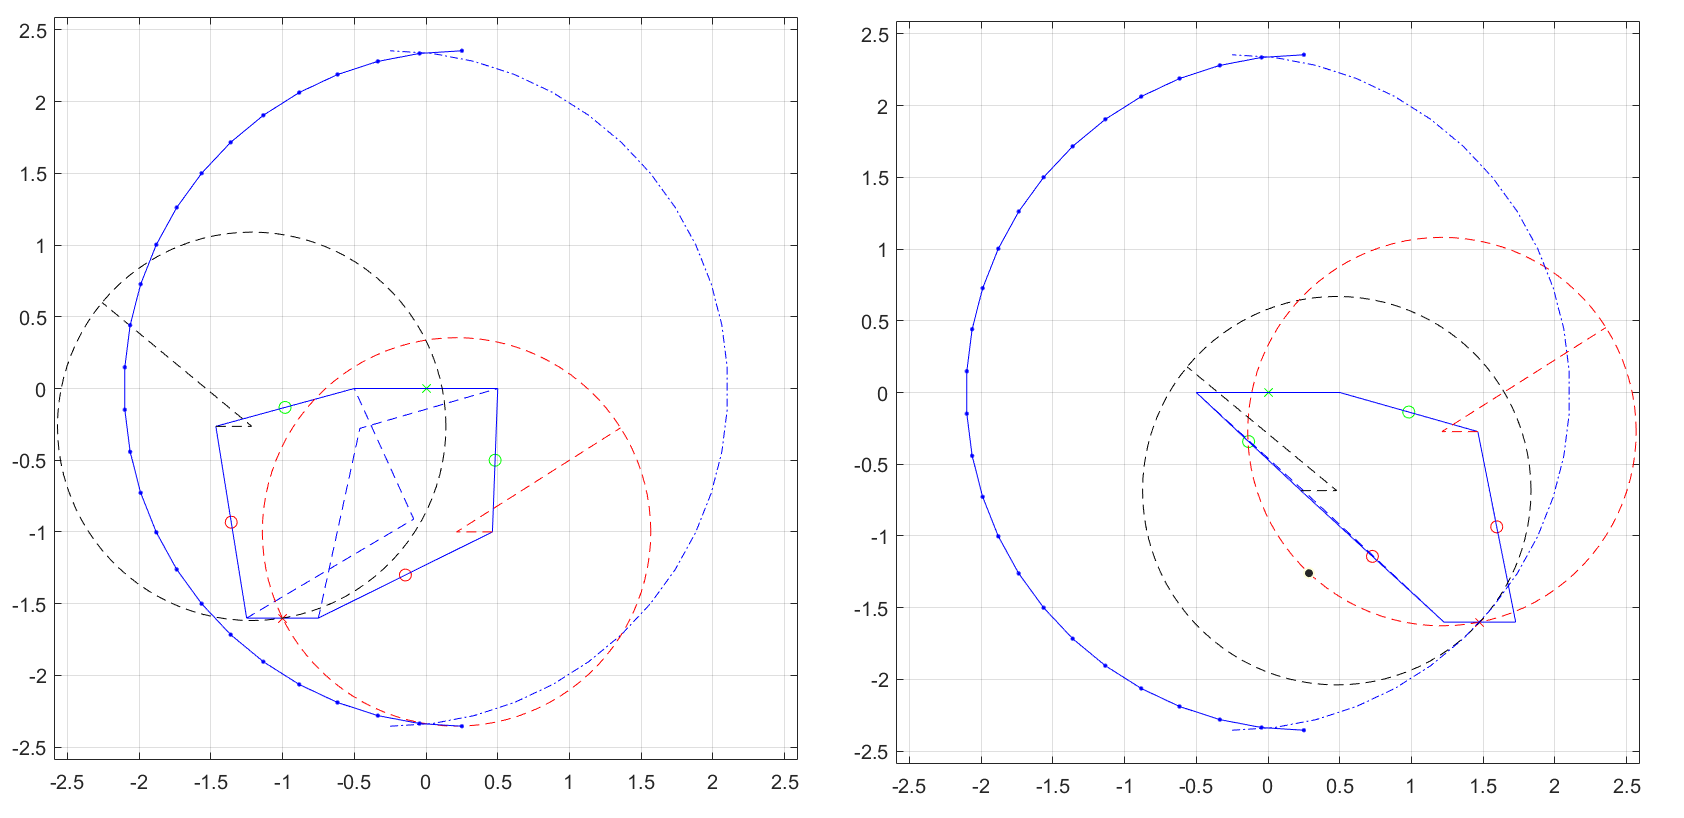
\includegraphics[width=\textwidth]{figures/Boundaries_2D.png}                                                     
	\caption[Interpretation of the inverse kinematics equation]{Interpretation of the inverse kinematics equation. The circles are centered at $x=\mp\tfrac{1}{2}L_b-L_u cos(\theta_{U,j})\pm\tfrac{1}{2}L_e$  and $y=-L_u sin(\theta_{U,j})$}
	\label{fig:inverse2D}
\end{figure}

By eliminating the dependent $x$ and $y$ co-ordinates in equation \ref{eq:Phi2D}, the following equations can be obtained:
\begin{equation}
    \Phi^{IK}=
    \begin{bmatrix}
     (\mp \frac{L_b}{2}-L_u cos(\theta_{U,j})\pm\frac{L_e}{2}-P_x)^2+(-P_y-L_u sin(\theta_{U,j}))^2-L_l^2 \\
         \vdots
    \end{bmatrix}
\end{equation}

%\begin{figure}[h!]
%	\centering
%	\includegraphics[width=0.7\textwidth]{figures/Inverse_2D_edge.png}                                                     
%	\caption[Fully extended arm]{Fully extended arm. The boundaries are shown with the 'dot-solid' and 'dot-dash' lines.}
%	\label{fig:inverse2D_edge}
%\end{figure}

The boundary is obtained by analysing the case where one arm is fully extended. That is, where $\theta_{U,j}=\theta_{L,j}$. See figure \ref{fig:inverse2D}.:
\begin{align*}
P_x&=\mp\tfrac{L_b}{2}-(L_u+L_l)cos(\theta_{U,j})\pm\tfrac{L_e}{2} \\
P_y&=-(L_u+L_l)sin(\theta_{U,j})
\end{align*}
Eliminating $\theta_{U,j}$:
\begin{equation}
(P_x\pm\tfrac{L_b}{2}\mp\tfrac{L_e}{2})^2+P_y^2=(L_u+L_l)^2
\end{equation}
The workspace is the intersection of the two circles. When $L_e=L_b$, the two circles will merge into one full circle.

\begin{align}
\Phi^{IK} =& 0  \nonumber \\
\implies \tfrac{d\Phi}{dt} =&\Phi_{q_i} \tfrac{dq_i}{dt}+\Phi_{P} \tfrac{dP}{dt}  =0\\
\implies 
\tfrac{d^2\Phi}{dt^2} =&([\Phi_{q_i}\tfrac{dq_i}{dt}]_{q_i}\tfrac{dq_i}{dt}+[\Phi_{q_i}\tfrac{dq_i}{dt}]_{P}\tfrac{dP}{dt})+\Phi_{q_i}\tfrac{d^2q_i}{dt^2}+ \nonumber\\
                           &([\Phi_{P}\tfrac{dP}{dt}]_{q_i}\tfrac{dq_i}{dt}+[\Phi_{P}\tfrac{dP}{dt}]_{P}\tfrac{dP}{dt})+\Phi_{P}\tfrac{d^2P}{dt^2}\hphantom{+}=0\\
\therefore  \tfrac{d^2q_i}{dt^2}=&-\Phi_{q_i}^{-1} (\Phi_{q_iq_i}\tfrac{dq_i}{dt}^2+\Phi_{PP}\tfrac{dP}{dt}^2+2\Phi_{q_iP}\tfrac{dq_i}{dt}\tfrac{dP}{dt}+\Phi_P\tfrac{d^2P}{dt}) \label{eq:gammaIK}
\end{align}

\subsection{Kinetics}
The Lagrange multiplier method has been used to calculate the forces. See \cite{Schilder2018} for more detail.\\

The primary equation is:
\begin{eqnarray}
M\ddot{q}+\Phi_q^T\lambda=Q_A \label{eq:lambda}
\end{eqnarray}
Where $Q_A$ are the applied forces and $\lambda$ the Lagrange multipliers. The $\lambda$ can be solved for directly if $\Phi_q$ has full rank, which will be the case if it kinematically driven. Otherwise, $\Phi_q$ will have more columns for co-ordinates $q$ than rows for constraint equations, and will not be invertible. They must then be solved for simultaneously with the accelerations:
\begin{equation}
\begin{bmatrix}
M &\Phi_q^T \\
\Phi_q &0
\end{bmatrix}
\begin{bmatrix}
\ddot{q} \\
\lambda
\end{bmatrix}
=
\begin{bmatrix}
Q_A \\
\gamma
\end{bmatrix} \label{eq:EoM}
\end{equation}
See the appendix for more detail.\\

Each $\lambda$ can be related to constraint forces at a particular point P from a centroid with co-ordinates $(X,Y,\Theta)$ with:
\begin{equation}
\begin{aligned}
F_{P,x}&=-\Phi_{P,X}^T\lambda_P \\
F_{P,y}&=-\Phi_{P,Y}^T\lambda_P \\
M_P    &=-\Phi_{P,\Theta}^T\lambda_P+y_{P/Y}-F_{P,x}-x_{P/X}F_{P,y}
\end{aligned}
\end{equation}
Where $\Phi_{P,\Theta}$ is the Jacobian of the relevant constraints at P with respect to $(X,Y,\Theta)$. Equivalently, it is the sub-matrix of $\Phi_q$ with the same indices as the relevant constraint equations and co-ordinates.\\

The constraint forces can also be found by solving:
\begin{equation}
\begin{aligned}
m_u \ddot{x}_u &= F_{A,x}+F_{B,x} \\ 
m_u \ddot{y}_u &= F_{A,y}+F_{B,y} -m_u g \\
I_u \ddot{\theta_u}&=-(F_{B,x}-F_{A,x})\tfrac{1}{2}L_usin(\theta_U)+(F_{B,y}-F_{A,y})\tfrac{1}{2}L_ucos(\theta_U)+M_a\\
m_l \ddot{x}_l &= -F_{B,x}+F_{C,x} \\ 
m_l \ddot{y}_l &= -F_{B,y}+F_{C,y} -m_l g\\
\end{aligned}
\end{equation}


References: \cite{Schilder2018} \cite{Hibbeler2013}
% \begin{align}
%     M_{ii}=
%     \begin{bmatrix}
%     I_{upper} & 0\\
%     0 & I_{upper} 
%     \end{bmatrix}
% \end{align}

